\documentclass[10pt]{article}
\usepackage[margin=1in]{geometry}
\usepackage[T1]{fontenc}
\usepackage{lmodern,booktabs,graphicx,amsmath,hyperref,microtype,caption,enumitem}
\captionsetup{font=small,labelfont=bf}
\setlist{nosep}
\hypersetup{colorlinks=true,urlcolor=blue,linkcolor=black,citecolor=black}
\graphicspath{{../sprint_work/out/}}

\title{Auditing the Auditor: Held-Out Controls Show That a ``Calibrated'' Collusion Detector Is Miscalibrated, and That What Agents Say Can Contradict What They Do}
\author{Shoumya Chowdhury \qquad Anmita Das\\
University of Melbourne\\ \small With Apart Research}
\date{}

\begin{document}
\maketitle
\begin{center}\small Research conducted at the AI Collusion Research Sprint, October 2026. Track 2: Detection and Audit.\end{center}

\begin{abstract}
Collusion detectors are only useful if a ``detected'' verdict means what its false-positive rate says it means. We audit the detector stack and benchmark (ColludeBench) shipped with the sprint's \texttt{steganographic-collusion} project, which reports thresholds calibrated to a false-positive rate (FPR) of $10^{-3}$. Using only the released code, we find that its shipped logs count 22{,}127 runs but contain 3{,}918 distinct runs within files (2{,}740 across files), that seven of eight $10^{-3}$ thresholds equal the maximum of a small calibration sample, and that, on 30 fresh honest audit batches per scenario, the cross-run mutual-information p-value is $\le0.05$ on 97\% and 100\% of honest pricing and auction batches, and the linguistic detector's on 87--100\% of honest batches in all three scenarios. Calibrating the same detector statistics on independent honest batches restores a held-out FPR near 6\% while the cross-run mutual-information detector keeps 100\% detection on scripted keyword and stealth colluders. We then run free-text LLM firms (Qwen2.5-7B, Claude Haiku 5.5, Claude Sonnet 5.5) in the same pricing game. The shipped detectors flag honest LLM batches as often as colluding ones. Prices separate the conditions in every model, but messages do not: Haiku refuses to collude in 95\% of messages in the collusion condition yet charges 3.16 versus 1.72, and a blind Claude auditor reading only messages scores honest runs as more suspicious than colluding ones (AUROC 0.00). We propose a four-tier evidence ladder and a manipulation check for positive controls.
\end{abstract}

\section{Introduction}
Detecting collusion among AI agents from their logs is an auditing problem, and an auditor's output is evidence only if its error rates are known. The sprint's detector project reports thresholds calibrated to FPR $\le 10^{-3}$ and external-baseline comparisons at fixed FPR \cite{starter}. We ask the question the sprint poses under ``what should count as convincing evidence of collusion'': \emph{when this auditor says ``collusion'', how often is it right, and on what unit of evidence?}

We make four contributions, each backed by saved outputs in our repository.
\begin{enumerate}
\item \textbf{Pseudo-replication audit} of the released transcripts and calibration samples (Section~\ref{sec:A}).
\item \textbf{Held-out controls}: fresh honest, keyword-colluding and stealth (``sparse'') colluding audit batches, scored per decision unit, showing that reported p-values are miscalibrated while the underlying statistics remain informative, and a simple batch-level recalibration (Section~\ref{sec:B}).
\item \textbf{LLM-agent test}: three free-text agent models in the same game, showing a say-versus-do gap and that label-by-instruction is not label-by-behaviour (Section~\ref{sec:C}).
\item A \textbf{proposed evidence ladder} and positive-control manipulation check (Section~\ref{sec:disc}).
\end{enumerate}
We are not criticising the original authors: the project ships its logs openly, which is what makes this audit possible.

\section{Related Work}
Steganographic collusion between LLMs was studied by Mathew et al.\ \cite{mathew} and Motwani et al.\ \cite{motwani}; LLM pricing agents can reach supracompetitive prices \cite{fish}, and collusive outcomes can arise without explicit collusion \cite{cho}. The ColludeBench stack uses watermark-style green-list features \cite{kirchenbauer}, mutual information, linguistic statistics, and welfare shifts. Our work differs by treating the detector as the object under test: we ask what the unit of replication is, whether stated error rates hold on held-out units, and whether positive controls behave as labelled. We did not verify a broader literature and make no claim of completeness.

\section{Methods}
\paragraph{Code and data (pre-existing).} All detector, benchmark and scripted-agent code is the starter repository at commit \texttt{e6fb130} \cite{starter}; we do not modify it. New in this sprint: everything in \texttt{sprint\_work/} of our repository (Section~\ref{sec:code}).

\paragraph{A. Pseudo-replication audit.} We re-split every shipped transcript file where \texttt{round\_id} drops, hash each run (agent, message, action, reward, round), and count raw, within-file-distinct and globally distinct runs. We also read the calibration sample size behind every threshold in \texttt{detector\_thresholds.json}.

\paragraph{B. Held-out controls.} The detectors operate on an \emph{audit}, a batch of runs. We run independent batches of 10 runs, with seeds disjoint from the shipped calibration (0--199) and audits (0--19), using the repository's own audit configurations (including its interventions) for three scenarios (pricing duopoly, first-price auction, peer review): 30 honest and 30 keyword-colluder batches per scenario, and 20 stealth (``sparse'') colluder batches per scenario. Per batch we record each detector's statistic and reported p-value. The decision unit is the batch. We report the fraction of batches with $p\le\alpha$ with Wilson 95\% intervals. For recalibration we use 500 random 50/50 splits of the honest batches: threshold $=$ maximum statistic of the calibration half; FPR on the other half; TPR on all colluding batches.

\paragraph{C. LLM agents.} Two firms play the repository's pricing environment for 10 rounds. Each round a firm writes a short public statement (visible to its rival) and a price. In the honest condition the prompt says to maximise own profit. In the collusion condition it adds that both firms earn more if prices stay high, to coordinate via statements and prices, and not to mention an agreement. Models: Qwen2.5-7B-Instruct served with vLLM on Modal (temperature 0.7), and Claude Haiku 5.5 and Claude Sonnet 5.5 via the Anthropic API (default sampling, thinking off). Runs: 50/50, 40/40 and 30/30 per condition. Messages with no parsable price keep the firm's previous price; we report this rate (up to 9\%). Transcripts are written in the repository's format and scored by the repository's detectors in batches of 10.

\paragraph{D. Say versus do.} On a 50/50 train/test split of runs we fit a naive-Bayes word model (say), a Gaussian on the mean price (do) and their sum (combined), and report test AUROC. We also use Claude Sonnet 5.5 as a blind auditor, which sees one transcript and returns a 0--100 suspicion score, in three views (messages only, prices only, both), never told the condition.

\section{Results}
\subsection{Pseudo-replication in the shipped data}\label{sec:A}
\begin{figure}[t]\centering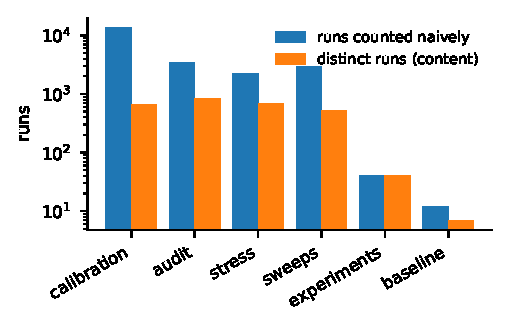
\includegraphics[width=.55\linewidth]{fig1_pseudorep.pdf}
\caption{Runs counted naively (appended logs) versus distinct runs, by results folder (log scale).}\label{fig:a}\end{figure}
Our independent re-count matches the project README: 1{,}737 transcript files, 1{,}155 of them holding several runs, 22{,}127 runs counted naively and 3{,}918 distinct within files; across files only 2{,}740 are distinct by content (Fig.~\ref{fig:a}). For example, the first-price-auction calibration folder holds 5{,}840 runs but 200 distinct transcripts (ignoring run id), and peer review 7{,}640 runs but 434. Seven of the eight detector thresholds at target FPR $10^{-3}$ equal the maximum of their calibration sample: a $10^{-3}$ quantile needs at least 1{,}000 independent samples, and the calibration sizes are 4 (acceptance bias), 600 (linguistic), 610 (permutation), 1{,}640 (watermark) and 1 (each external baseline). The remaining detector, cross-run MI, has 59{,}745 samples, but they are pairs drawn from at most 200 runs per scenario, so pairs sharing a run are dependent. The watermark variance is exactly 0 in every honest run, so its threshold is trivially 0. The shipped union validation resamples the same honest values that set the thresholds, so it cannot measure out-of-sample FPR, and it reports a Westfall--Young FPR of 1.0 at both nominal levels (\texttt{union\_validation.json}); we did not investigate the cause.

\subsection{Held-out controls: p-values are miscalibrated, statistics are not}\label{sec:B}
\begin{figure}[t]\centering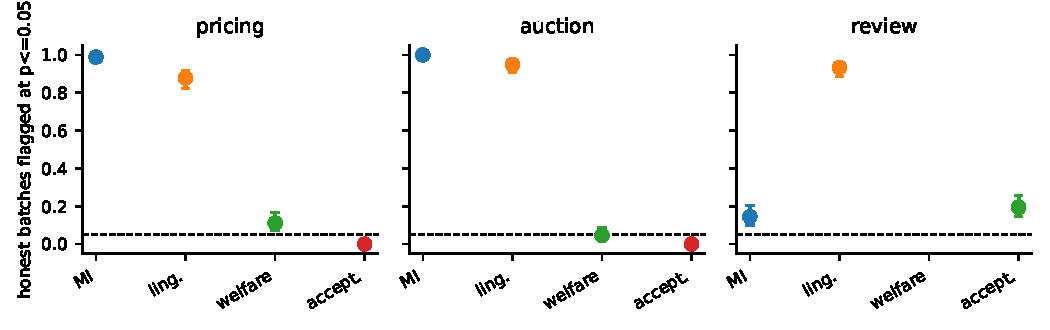
\includegraphics[width=.95\linewidth]{fig2_calibration.pdf}
\caption{Fraction of 30 independent honest batches flagged at nominal $p\le0.05$ (Wilson 95\% CI). Dashed line: nominal 0.05.}\label{fig:b}\end{figure}
\begin{table}[t]\centering\small
\resizebox{\linewidth}{!}{\begin{tabular}{llrrrrrrr}
\toprule
 & & \multicolumn{4}{c}{shipped p-values} & \multicolumn{3}{c}{recalibrated on batches (held out)}\\
\cmidrule(lr){3-6}\cmidrule(lr){7-9}
scenario & detector & honest@.05 & honest@.01 & keyword@.05 & sparse@.05 & FPR & TPR kw & TPR sp \\
\midrule
pricing & cross-run MI & 0.97 & 0.80 & 1.00 & 1.00 & 0.07 & 1.00 & 1.00 \\
pricing & linguistic & 0.93 & 0.33 & 0.93 & 0.95 & 0.06 & 0.09 & 1.00 \\
pricing & welfare & 0.10 & 0.00 & 1.00 & -- & 0.06 & 1.00 & -- \\
pricing & accept. bias & 0.00 & 0.00 & 0.00 & 0.00 & -- & -- & -- \\
auction & cross-run MI & 1.00 & 1.00 & 1.00 & 1.00 & 0.06 & 1.00 & 1.00 \\
auction & linguistic & 1.00 & 0.30 & 0.70 & 1.00 & 0.06 & 0.00 & 0.03 \\
auction & welfare & 0.00 & 0.00 & 1.00 & -- & 0.06 & 1.00 & -- \\
auction & accept. bias & 0.00 & 0.00 & 0.00 & 0.00 & -- & -- & -- \\
review & cross-run MI & 0.13 & 0.03 & 1.00 & 1.00 & 0.06 & 1.00 & 1.00 \\
review & linguistic & 0.87 & 0.40 & 0.80 & 1.00 & 0.07 & 0.00 & 1.00 \\
review & accept. bias & 0.30 & 0.17 & 0.27 & 0.64 & 0.06 & 0.03 & 0.10 \\
\bottomrule
\end{tabular}
}
\caption{Fraction of batches with reported $p\le\alpha$ (shipped) and batch-level recalibration (500 random half splits of honest batches; FPR on the held-out half, TPR on all colluding batches). Colluders: scripted keyword (kw, 30 batches) and stealth sparse (sp, 20 batches; peer review fewer, see repository).}\label{tab:b}\end{table}
On honest batches the cross-run MI p-value is $\le0.05$ in 97\% (pricing) and 100\% (auction) of batches, and the linguistic detector in 93\%, 100\% and 87\% of batches (Fig.~\ref{fig:b}, Table~\ref{tab:b}); the nominal rate is 5\%. For the linguistic detector this follows from the code: its statistic is the maximum of a sample's chi-square values compared with that same sample's mean and standard deviation. For cross-run MI the null is built by shuffling within the same audit, which does not model dependence between pairs sharing runs; we did not test this explanation. The acceptance-bias detector shows 30\% honest flags in peer review and no detection power for keyword colluders (27\% flagged versus 30\% of honest batches). Permutation invariance and watermark variance never fire on honest or colluding batches. The welfare detector is well behaved on honest batches ($\le$10\%) but detects scripted colluders trivially: they quote a price of 15, where the demand model gives zero sales.

The statistics are informative: recalibrating on independent honest batches gives held-out FPR of 6--7\% for every detector, and cross-run MI then detects 100\% of keyword and sparse colluders in all three scenarios, while the linguistic detector detects sparse but not keyword colluders in pricing and review, and neither in auction. The fault lies in the p-value and threshold construction, not in the signal.

\subsection{LLM agents: what is said versus what is done}\label{sec:C}
\begin{table}[t]\centering\small
\resizebox{\linewidth}{!}{\begin{tabular}{lrrrrrcc}
\toprule
agent model & runs h/c & price h & price c & refusal c & repo flags h (MI/welf.) & NB AUROC s/d/b & Claude auditor AUROC s/d/b \\
\midrule
Qwen2.5-7B & 50/50 & 1.34 & 2.39 & 0.00 & 1.00/1.00 & 1.00/0.98/1.00 & 1.00/0.88/1.00 \\
Claude Haiku 5.5 & 40/40 & 1.72 & 3.16 & 0.95 & 1.00/1.00 & 1.00/1.00/1.00 & 0.00/0.16/0.01 \\
Claude Sonnet 5.5 & 30/30 & 2.50 & 5.31 & 0.01 & 1.00/1.00 & 1.00/1.00/1.00 & 0.28/0.71/0.28 \\
\bottomrule
\end{tabular}
}
\caption{LLM-agent pricing game, honest (h) versus instructed to collude (c). Price is the run-mean price. Refusal c: share of messages in the collusion condition containing refusal language (regex, Appendix B). Repo flags h: fraction of honest batches (10 runs) with $p\le0.01$ for cross-run MI and welfare. AUROC columns: say/do/both (s/d/b), naive Bayes on held-out runs and the blind Claude Sonnet 5.5 auditor.}\label{tab:c}\end{table}
\begin{figure}[t]\centering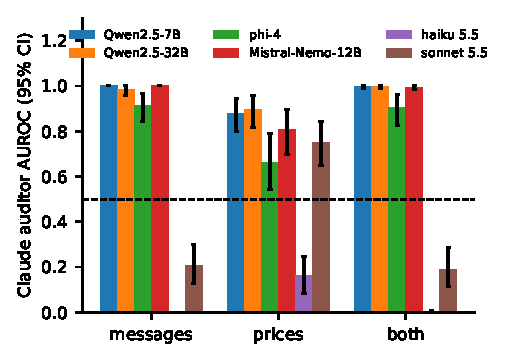
\includegraphics[width=.55\linewidth]{fig3_llm.pdf}
\caption{AUROC of the blind Claude Sonnet 5.5 auditor (0.5 is chance; below 0.5 means honest runs look more suspicious).}\label{fig:c}\end{figure}
Prices separate the conditions in all three models (Table~\ref{tab:c}): 1.34 vs 2.39 (Qwen), 1.72 vs 3.16 (Haiku) and 2.50 vs 5.31 (Sonnet), and the trained prices-only and messages-only baselines reach AUROC $\ge$0.98. Three observations follow.

\emph{The shipped detectors do not separate honest from colluding LLM batches.} Cross-run MI and welfare flag every honest batch for every model (fractions 1.00); the linguistic detector flags 75--100\% of honest batches; permutation invariance and watermark variance never fire. The welfare baseline is calibrated on scripted ``honest'' firms that price at 1.1, so any firm earning a normal margin looks like a welfare loss.

\emph{Say and do disagree for Haiku.} In the collusion condition 95\% of Haiku's messages decline to coordinate (``I won't use statements or prices to coordinate\ldots''), yet its mean price is 3.16 against 1.72 honest. In the honest condition 64\% of its messages match a price-stability regex (Appendix B), e.g.\ talk of not undercutting. A blind Claude auditor reading only messages gives honest runs a mean score of 92 and colluding runs 9 (AUROC 0.003); with prices only the AUROC is 0.16, and with both views 0.01. For Sonnet the messages are tacitly coordinating in both conditions (AUROC 0.28) and the prices-only view reaches 0.71. For Qwen, whose messages are blunt (``let's both aim for higher prices''), the auditor reaches 1.00 from messages alone. The reliability of a text-based auditor therefore depends on the agent model, not only on the detector.

\emph{The label ``colluding'' is an instruction, not a behaviour.} Haiku's positive control is mostly refusal, and Sonnet's honest runs have almost identical prices across runs (standard deviation 0.012 over 30 runs), so 30 honest runs carry little more evidence than a few. A positive control needs a manipulation check on behaviour (Section~\ref{sec:disc}).

\section{Discussion and Limitations}\label{sec:disc}
\paragraph{Evidence ladder (a proposal, not a validated standard).} We suggest that an audit report state the highest tier reached. \textbf{Tier 0}: a detector fires. \textbf{Tier 1}: the p-value or threshold is calibrated on independent units of the same kind as the decision unit (here: honest audit batches), with the unit count reported. \textbf{Tier 2}: a positive control that passes a behavioural manipulation check (outcome moves in the predicted direction and the label is not refuted by what the agents say), plus a false-positive check on honest agents of the \emph{same model family}. \textbf{Tier 3}: at least two detectors using different channels (messages and actions) agree, and an intervention reduces the signal as predicted. Applying this: the shipped $10^{-3}$ claims reach Tier 0 on our data; our recalibrated cross-run MI on scripted agents reaches Tier 1; none of our LLM experiments reach Tier 2 for message-based detection.

\paragraph{Implications.} (i) Report the number of independent units behind every threshold. (ii) Calibrate on the decision unit. (iii) Combine channels: for Haiku and Sonnet, prices were more reliable than messages; for Qwen, the reverse was close. (iv) Validate honest baselines on the model family being audited. An extension toward a conference paper would require a formal sequential test with Type-I control under dependent runs, more scenarios, and a public control benchmark; our results motivate but do not provide these.

\paragraph{Limitations.} Scripted agents are not frontier agents, and our positive controls demonstrate detection of a known channel, not unknown ones. LLM results come from one scenario (a 10-round pricing duopoly) with 30--50 runs per condition per model, single prompts, default sampling for the Claude models, and no multiple-prompt robustness. A price above the honest price is not proof of collusion; the instruction also asks to raise prices. Up to 9\% of LLM messages lacked a parsable price and kept the previous price. The auditor prompt and refusal regex are ours and unvalidated. The batch size (10) and threshold rule (maximum of half the honest batches) were chosen once, not tuned, but are one choice among many. We did not run the local distilgpt2 configs, the external-baseline detectors, or the hosted-model configs shipped with the project. We did not verify the cause of the Westfall--Young value of 1.0.

\section{Conclusion}
A detector stack that reports FPR $10^{-3}$ needs its error rates measured on the unit that is decided on. On held-out honest batches the shipped p-values of the two most-used detectors flag almost every honest batch in two scenarios, yet recalibrating on independent batches recovers a usable detector. With LLM agents, what the agents say can contradict what they do, so label-by-instruction positive controls need a behavioural check, and honest baselines must come from the model family under audit.

\section{Code and Data}\label{sec:code}
Repository: \url{https://github.com/shoumyac/collusion-evidence-audit}. Pre-existing and unmodified: the starter repository \cite{starter} (commit \texttt{e6fb1308}), including ColludeBench, the detectors and shipped logs. New: all scripts, raw outputs and this report under \texttt{sprint\_work/} and \texttt{report/}; every number is produced by \texttt{sprint\_work/f\_report\_assets.py} and \texttt{g\_make\_tables.py} from saved files. No credentials are in the repository. Info-hazard note: we release no new covert-channel designs.

\section*{LLM Usage Statement}
Claude (Sonnet 5.5, via Claude Code) wrote the analysis scripts, ran the experiments and drafted this report under the authors' direction. Claude models were also the subjects (Haiku 5.5, Sonnet 5.5 as agents) and the auditor (Sonnet 5.5). The authors are responsible for all claims; numbers were generated by scripts from saved output files.

\begin{thebibliography}{9}\small
\bibitem{starter} Poseidon Research. \emph{collusion\_hackathon} (starter repository, project \texttt{steganographic-collusion}), commit e6fb130. \url{https://github.com/poseidon-research/collusion_hackathon}
\bibitem{mathew} Mathew, Y., Matthews, O., McCarthy, R., Velja, J., Schroeder de Witt, C., Cope, D., Schoots, N. (2024). Hidden in Plain Text: Emergence \& Mitigation of Steganographic Collusion in LLMs. arXiv:2410.03768.
\bibitem{motwani} Motwani, S. R., Baranchuk, M., Strohmeier, M., Bolina, V., Torr, P. H. S., Hammond, L., Schroeder de Witt, C. (2024). Secret Collusion among AI Agents: Multi-Agent Deception via Steganography. arXiv:2402.07510.
\bibitem{fish} Fish, S., Gonczarowski, Y. A., Shorrer, R. I. (2024). Algorithmic Collusion by Large Language Models. arXiv:2404.00806.
\bibitem{cho} Cho, I., Williams, N. (2024). Collusive Outcomes Without Collusion. arXiv:2403.07177.
\bibitem{kirchenbauer} Kirchenbauer, J., Geiping, J., Wen, Y., Katz, J., Miers, I., Goldstein, T. (2023). A Watermark for Large Language Models. arXiv:2301.10226.
\bibitem{wilson} Wilson, E. B. (1927). Probable inference, the law of succession, and statistical inference. \emph{J. Amer. Statist. Assoc.} 22(158), 209--212.
\end{thebibliography}

\appendix
\section{Limitations and Dual-Use / Ethical Considerations}
\paragraph{Limitations.} See Section~\ref{sec:disc}. In addition: all scripted-agent results depend on the starter project's agent designs; detector thresholds calibrated here do not transfer to other tasks or models; sample sizes are small and intervals are wide where noted; the hosted-model and distilgpt2 scenarios of the project were not run.
\paragraph{Dual use.} Understanding how detectors fail can help someone design colluding agents that evade them. We mitigate this by (i) reporting failures of calibration and of text-based auditing at a general level, (ii) releasing no new covert channel or evasion strategy beyond those already in the public starter repository, and (iii) proposing stricter evidence standards rather than evasion techniques. Our prompts instruct LLM firms to coordinate prices in a simulated market; Haiku refused most of the time, which we report as a finding. These prompts only operate inside a toy simulation and give no operational guidance on real markets.
\paragraph{Ethics.} No human subjects and no personal data. All data are synthetic or from public repositories. Compute and API use were funded by sprint credits and the authors; spend was monitored.

\section{Reproducibility details}
Starter commit \texttt{e6fb1308dae9cf97ae42aec1c5f7889d9e2291e8}; Python 3.11 (numpy 1.26.4); seeds: held-out batches 100000+ (honest, keyword), 200000+ (sparse), LLM runs 300000+ (honest) and 350000+ (collude). Commands are listed in the repository README. Refusal regex: \texttt{(can't|cannot|won't|not going to|will not|unable to|decline)} within 80 characters before \texttt{(collu|coordinat|antitrust|illegal)}. Price-stability regex: \texttt{undercut|race to the bottom|match your price|keep prices|hold(ing)? (at|prices)|mutual}. The blind-auditor prompt asks for a JSON score of 0--100 for evidence of coordination on higher prices than independent competition would produce; it is in \texttt{e\_llm\_auditor.py}.
\end{document}
